\documentclass[tikz,border=3pt]{standalone}
% Shared preamble for every TikZ figure in the report.
% Colours are Okabe-Ito, with roles fixed across all nine figures.
\usepackage[T1]{fontenc}
\usepackage{lmodern}
\usepackage{amsmath,amssymb}
\usetikzlibrary{arrows.meta,positioning,calc,fit,backgrounds,shapes.geometric,shapes.misc,decorations.pathreplacing,patterns}

\definecolor{cGraph}{HTML}{0072B2}
\definecolor{cSem}{HTML}{E69F00}
\definecolor{cFuse}{HTML}{009E73}
\definecolor{cLoop}{HTML}{D55E00}
\definecolor{cOracle}{HTML}{CC79A7}
\definecolor{cNeutral}{HTML}{999999}
\definecolor{cInk}{HTML}{222222}

\tikzset{
  every picture/.style={line width=0.5pt},
  box/.style={draw=cNeutral!90!black, fill=cNeutral!8, rounded corners=1.6pt,
              align=center, inner sep=3.2pt, font=\small, text=cInk},
  gbox/.style={box, draw=cGraph, fill=cGraph!7},
  sbox/.style={box, draw=cSem!80!black, fill=cSem!12},
  fbox/.style={box, draw=cFuse, fill=cFuse!8},
  lbox/.style={box, draw=cLoop, fill=cLoop!8},
  ann/.style={font=\scriptsize, text=cInk, align=center, inner sep=1.5pt},
  flow/.style={-{Stealth[length=4pt,width=3.2pt]}, draw=cNeutral!85!black},
  gflow/.style={flow, draw=cGraph},
  sflow/.style={flow, draw=cSem!85!black},
}

% Figure labels are short; never hyphenate them.
\hyphenpenalty=10000
\exhyphenpenalty=10000

\begin{document}
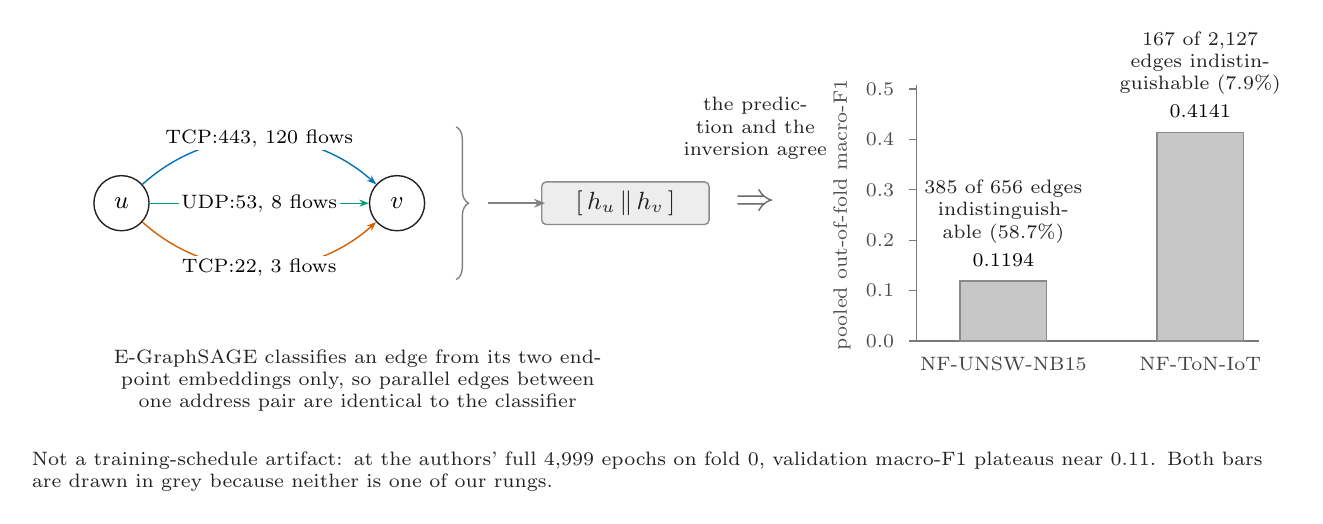
\begin{tikzpicture}[x=1cm,y=1cm]

% ================================================== left: the mechanism
\node[circle, draw=cInk, fill=white, minimum size=7mm, font=\small] (u) at (0.9,1.55) {$u$};
\node[circle, draw=cInk, fill=white, minimum size=7mm, font=\small] (v) at (4.4,1.55) {$v$};

\draw[-{Stealth[length=3.4pt]}, draw=cGraph, bend left=42] (u) to
      node[font=\scriptsize, fill=white, inner sep=1pt]{TCP:443, 120 flows} (v);
\draw[-{Stealth[length=3.4pt]}, draw=cFuse]              (u) to
      node[font=\scriptsize, fill=white, inner sep=1pt]{UDP:53, 8 flows} (v);
\draw[-{Stealth[length=3.4pt]}, draw=cLoop, bend right=42] (u) to
      node[font=\scriptsize, fill=white, inner sep=1pt]{TCP:22, 3 flows} (v);

\node[box, fill=cNeutral!18, draw=cNeutral!90!black, text width=1.9cm] (hh) at (7.30,1.55)
      {$[\,h_u \,\|\, h_v\,]$};
\draw[decorate, decoration={brace, mirror, amplitude=4.5pt}, draw=cNeutral!85!black]
      (5.15,0.58) -- (5.15,2.52);
\draw[flow, draw=cNeutral!85!black, line width=0.9pt] (5.55,1.55) -- (6.28,1.55);

\node[ann, anchor=north, text width=8.0cm] at (3.9,-0.25)
      {E-GraphSAGE classifies an edge from its two endpoint embeddings only, so parallel
       edges between one address pair are identical to the classifier};

% ================================================== the bridge
\node[font=\Large, text=cInk!70] at (8.95,1.55) {$\Rightarrow$};
\node[ann, anchor=south, text width=2.2cm] at (8.95,2.05)
      {the prediction and the inversion agree};

% ================================================== right: the confirmation
\def\ax{11.00}\def\ay{-0.20}\def\sc{6.4}     % 0.5 macro-F1 maps to 3.2 cm
\draw[draw=cInk!60] (\ax,\ay) -- (\ax,\ay+3.25);
\draw[draw=cInk!60] (\ax,\ay) -- (15.35,\ay);
\foreach \t in {0.0,0.1,0.2,0.3,0.4,0.5}{
  \draw[draw=cInk!60] (\ax,{\ay+\t*\sc}) -- (\ax-0.10,{\ay+\t*\sc});
  \node[font=\scriptsize, anchor=east, text=cInk!80] at (\ax-0.16,{\ay+\t*\sc}) {\t};
}
\node[rotate=90, font=\scriptsize, text=cInk!80] at (\ax-0.95,{\ay+1.60})
      {pooled out-of-fold macro-F1};

\draw[fill=cNeutral!55, draw=cNeutral!90!black] (11.55,\ay) rectangle (12.65,{\ay+0.1194*\sc});
\draw[fill=cNeutral!55, draw=cNeutral!90!black] (14.05,\ay) rectangle (15.15,{\ay+0.4141*\sc});
\node[font=\scriptsize, anchor=south] at (12.10,{\ay+0.1194*\sc+0.06}) {0.1194};
\node[font=\scriptsize, anchor=south] at (14.60,{\ay+0.4141*\sc+0.06}) {0.4141};
\node[font=\scriptsize, anchor=north, text=cInk!85] at (12.10,\ay-0.08) {NF-UNSW-NB15};
\node[font=\scriptsize, anchor=north, text=cInk!85] at (14.60,\ay-0.08) {NF-ToN-IoT};

\node[ann, anchor=south, text width=2.3cm] at (12.10,{\ay+0.1194*\sc+0.42})
      {385 of 656 edges indistinguishable ($58.7\%$)};
\node[ann, anchor=south, text width=2.3cm] at (14.60,{\ay+0.4141*\sc+0.42})
      {167 of 2{,}127 edges indistinguishable ($7.9\%$)};

% ================================================== footnote
\node[ann, anchor=north west, text width=15.8cm, align=left] at (-0.30,-1.55)
      {Not a training-schedule artifact: at the authors' full 4{,}999 epochs on fold 0,
       validation macro-F1 plateaus near 0.11. Both bars are drawn in grey because neither
       is one of our rungs.};

\end{tikzpicture}
\end{document}
